\section{Motivation}\label{motivation}

As described previously in \autoref{analysis-of-existing-synthesizers}, with the notable exceptions of VMPOP
\cite{parkTREDEVMPOPCultivating2018} and ForTrace
\cite{gobelForTraceHolisticForensic2022}, no synthesizer has been an
extension of another synthesizer. This raises the question -- why
reinvent the wheel by developing yet another distinct architecture for
this thesis? This section briefly explores the deficiencies in existing
synthesizers and explains why these are issues that warrant building a
new architecture from scratch rather than extending an existing
synthesizer.

The motivations for developing entirely new codebases instead of
extending existing synthesizers have varied considerably. One reason is
that several synthesizers are not open source and thus cannot easily be
extended, as is the case with Forensig2
\cite{mochForensicImageGenerator2009} and TraceGen
\cite{duTraceGenUserActivity2021}. Another reason is that the focus
of certain synthesizers results in an architecture that is simply
incompatible with the goals of newer works. For example, ForGe's
architecture \cite{vistiAutomaticCreationComputer2015} focuses
largely on direct filesystem manipulation to generate forensic artifacts
and is unsuitable for a synthesizer requiring virtualization. Similarly,
synthesizers that exclusively leverage agentless artifact generation as
described in \autoref{agentless-artifact-generation}, such as VMPOP \cite{parkTREDEVMPOPCultivating2018},
require significant architectural changes to support agent-based
artifact generation.

However, perhaps the largest motivation for constructing new
synthesizers is the lack of ongoing support for virtually all
synthesizers. It appears that no synthesizer has gained significant
traction within the broader forensic community, possibly with the
exception of ForTrace; for the synthesizers that \emph{are} open source,
none are under active development and maintenance. Additionally, the
forensic datasets generated by these synthesizers have not seen
significant adoption in either education or research; many instructors
continue to use the human-generated datasets available on public
platforms.

The inflexibility of prior synthesizers, combined with the overall lack
of support and success of synthesizer-based datasets, contributes to the
lack of shared codebases. However, this is not to say that the
individual contributions of each prior synthesizer cannot be merged into
a single project that resolves many of the architectural barriers that
have limited the adoption and extension of existing synthesizers.

In turn, the \emph{automated kinetic framework} (AKF) is built on the
following four pillars to help promote its long-term usage. In
particular, these design principles allow it to generate datasets that
address several of the considerations raised by Horsman and Lyle in the
construction of various datasets, such as the need for comprehensive
documentation, an awareness of the ``realism'' of the resulting dataset,
and transparency in the scenario development process
\cite{horsmanDatasetConstructionChallenges2021}.

First, AKF conforms to modern Python development practices. This
includes the use of modern project management practices (such as the use
of \passthrough{\lstinline!uv!} \cite{AstralshUv2025} and
\passthrough{\lstinline!pyproject.toml!}, rather than the use of
\passthrough{\lstinline!setup.py!} observed in older synthesizers),
static linters (\passthrough{\lstinline!flake8!}
\cite{PyCQAFlake82025}), and style enforcers
(\passthrough{\lstinline!black!}
\cite{langaBlackUncompromisingPython2025} and
\passthrough{\lstinline!isort!} \cite{PyCQAIsort2025}) to promote
adherence to the PEP8 standard. Additionally, AKF's libraries make heavy
use of Python 3.11+ features, including type hinting and special type
annotations, which allow for tools such as
\passthrough{\lstinline!mypy!} \cite{PythonMypy2025} to perform
static type checking. In addition to significantly improving the
development experience for new contributors, these practices also
increase the likelihood of discovering errors earlier in the development
process.

Second, AKF takes a modular, agent-based approach to implementing
application-specific functionality. This allows AKF to use existing
automation frameworks for web browsers and other applications, greatly
simplifying the codebase when compared to the implementation of the same
features in other synthesizers. This focus on flexibility makes it
significantly easier to install the agent, implement new
application-specific features, and more. This is a critical design
focus, given AKF's dependence on agents for most of its
application-specific functionality.

Third, AKF is architected to maintain feature parity with most prior
synthesizers. That is, although AKF deviates considerably from the
implementation details of prior synthesizers, this does not come at the
loss of prior advancements in the field. In particular, AKF supports all
three artifact generation techniques described in \autoref{chapter-four} using hypervisor-agnostic interfaces, reducing the tight
coupling that made certain features challenging to implement across
different synthesizers. This reduces the likelihood that a new feature
or technique will require a significant architectural change to support
it.

Finally, AKF is designed with the explicit intent of developing an
ecosystem of AKF-generated datasets, promoting long-term usage. This is
reflected in the design of AKF's logging and reporting mechanisms as
described in \autoref{chapter-five}; the use of an
RDF-based standard, CASE, allows for arbitrarily complex queries against
AKF datasets. These queries can be made in bulk, significantly improving
the ability of researchers to find and use datasets that may be relevant
to them.

These four pillars are reflected throughout the design of AKF's
architecture, which is described in the following section and the
following three chapters of this thesis.

\section{The AKF architecture}\label{the-akf-architecture}

At a minimum, every synthesizer must fulfill these high-level
requirements through some means, derived mainly from the criteria
developed by Horsman and Lyle
\cite{horsmanDatasetConstructionChallenges2021}:

\begin{itemize}
\tightlist
\item
  The synthesizer must accept commands on how it should operate. These
  commands should serve as a form of self-documentation, in which it is
  clear to another person \emph{what} the expected contents of the image
  are, as well as the \emph{intent} behind these commands.
\item
  The synthesizer must be able to accept external inputs, such as files
  and other binary data, to be used as part of artifact and dataset
  generation.
\item
  The synthesizer must implement the mechanisms and technologies
  necessary to carry out the commands it has been provided -- that is,
  it must be able to generate artifacts. Such mechanisms should be
  independently verifiable and leave as little extraneous information as
  possible.
\item
  The synthesizer must be able to generate a final output (such as a
  disk image), along with ground truth and reporting that describes the
  expected contents of that image. This should include a well-structured
  description of the dataset, a unique identifier, and explicit labels
  applied to data of ``evidential value'' where possible.
\end{itemize}

These four requirements are fulfilled by various mechanisms throughout
AKF. Detailed architectural diagrams can be seen in \autoref{appendix-a}, but a simplified diagram of AKF's top-level
``modules'' is shown in \autoref{fig:architecture-simple}.

\begin{figure}[h]
\centering
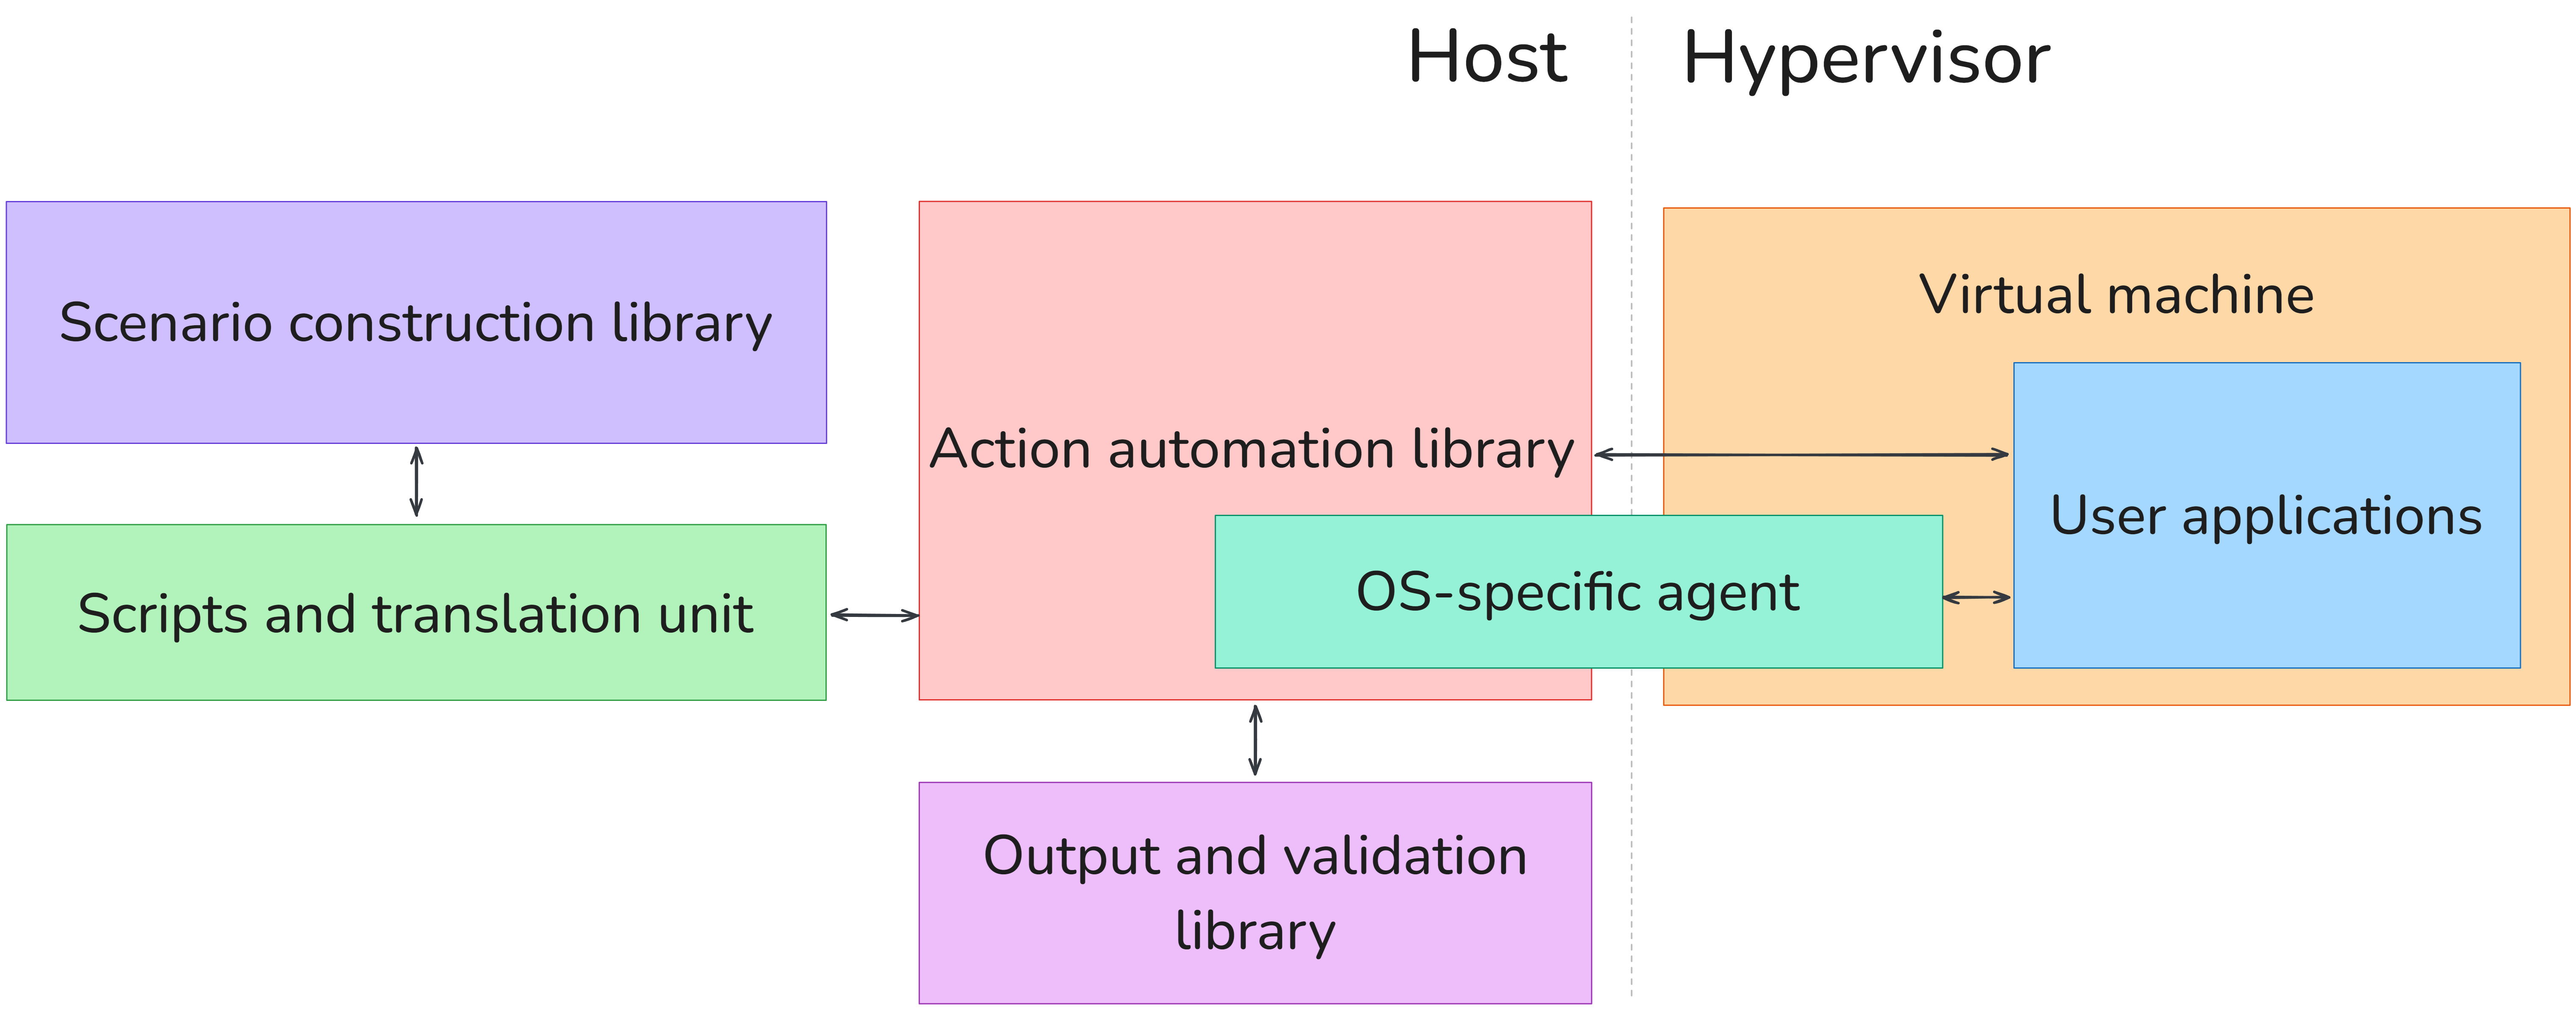
\includegraphics[width=1\linewidth]{architecture-simple.png}
\caption{Simplified AKF architecture
diagram}\label{fig:architecture-simple}
\end{figure}

AKF's seven top-level modules can be grouped into three distinct
concepts, each covering a specific chapter.

The first set of modules is responsible for artifact generation. This
encompasses three major systems - a hypervisor and its associated SDK,
an OS-specific agent, and \passthrough{\lstinline!akflib!}.
\passthrough{\lstinline!akflib!} is a Python library containing the
abstract interfaces and concrete implementations necessary to generate
artifacts and datasets. This includes routines for directly interacting
with hypervisors, issuing commands to virtual machines, and directly
modifying disk images. This library is also the foundation for
OS-specific agents, which carry out actions on the virtual machine on
behalf of the host. These modules are described in greater detail in
\autoref{chapter-four} and correspond to the \emph{action
automation library}, the \emph{OS-specific agent}, and the \emph{virtual
machine} (as well as the \emph{user applications} running on the
machine).

The second set of modules is responsible for logging and reporting. This
encompasses independent libraries for generating outputs and ground
truth, as well as the various logging-related mechanisms contained
throughout the artifact generation libraries. These modules are
responsible for exporting and documenting artifacts generated by AKF; in
particular, they make heavy use of CASE, a standardized ontology for
documenting the contents of forensic datasets
\cite{caseyAdvancingCoordinatedCyberinvestigations2017}. This is
covered in \autoref{chapter-five} and corresponds to the
\emph{output and validation library} and any associated components
within the \emph{action automation library}.

The final set of modules is responsible for invoking AKF itself and
supporting scenario development. AKF is an \emph{imperative}
synthesizer, which means that commands are written and executed using an
imperative language (Python 3) that dictates precisely \emph{how}
artifacts should be created. However, AKF also supports a
\emph{declarative} syntax, which allows users to specify \emph{what}
forensic artifacts should be generated without the need to understand
the AKF libraries and write actual Python code. These are discussed in
\autoref{chapter-six} and covers the \emph{scenario
construction library}, the \emph{translation unit}, and any scripts that
leverage AKF libraries. We also discuss the use of generative AI tools
for constructing individual artifacts and declarative scenarios.

The following three chapters will focus on these module groups. In
simpler terms, this thesis addresses the following questions in order:

\begin{itemize}
\tightlist
\item
  How do we automate or streamline the generation of artifacts?
\item
  How do we document and report on the artifacts and datasets that are
  generated?
\item
  Given the solutions that address these two questions, how do we
  actually use them to build scenarios?
\end{itemize}
